% Begin the document and set up the style of the document
\documentclass[a4paper]{article}

% Install the required packages for the document 
\usepackage{envmath}
\usepackage{esvect}
\usepackage{graphicx}
\usepackage{gensymb}
\usepackage{tikz}
\usepackage{geometry}
\usepackage{enumitem}
\usepackage{mathtools}
\usepackage{graphicx}
\usepackage{amsmath}
\usepackage{amscd}
\usepackage{amssymb}
\usepackage{amsfonts}
\usepackage{pgf}
\usepackage{tikz}
\usepackage{mathrsfs}
\usepackage{asyalign}
\usepackage{physics}
\usepackage{cite}
\usepackage{url}
\usepackage[tableposition=top]{caption}
\usepackage{ifthen}
\usepackage[utf8]{inputenc}
\usetikzlibrary{arrows}

\newcommand{\ds}{\displaystyle}

\begin{document}

\begin{center}
	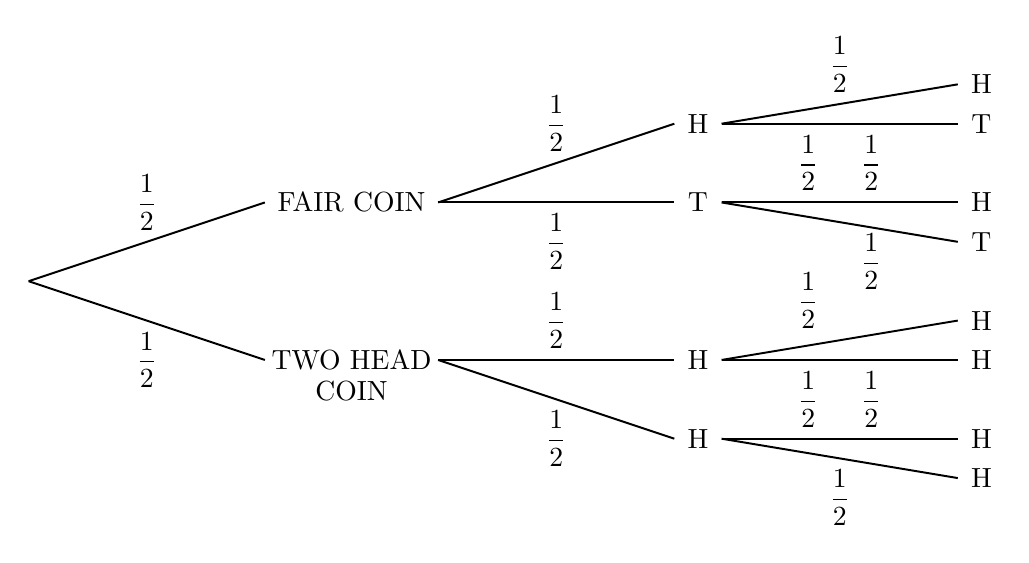
\begin{tikzpicture}

		\draw[line width = 0.25mm] (-4.5,0) -- (-1.5,1);
		\draw[line width = 0.25mm] (-4.5,0) -- (-1.5,-1);
		\node at (-0.4,1) {FAIR COIN};
		\node at (-0.4,-1) {TWO HEAD};
		\node at (-0.4,-1.4) {COIN};

		\draw[line width = 0.25mm] (0.7,1) -- (3.7,2);
		\draw[line width = 0.25mm] (0.7,-1) -- (3.7,-2);
		\draw[line width = 0.25mm] (0.7,1) -- (3.7,1);
		\draw[line width = 0.25mm] (0.7,-1) -- (3.7,-1);
		\node at (4,2) {H};
		\node at (4,1) {T};
		\node at (4,-1) {H};
		\node at (4,-2) {H};

		\draw[line width = 0.25mm] (4.3,2) -- (7.3,2.5);
		\draw[line width = 0.25mm] (4.3,2) -- (7.3,2);
		\draw[line width = 0.25mm] (4.3,1) -- (7.3,1);
		\draw[line width = 0.25mm] (4.3,1) -- (7.3,0.5);
		\draw[line width = 0.25mm] (4.3,-2) -- (7.3,-2.5);
		\draw[line width = 0.25mm] (4.3,-2) -- (7.3,-2);
		\draw[line width = 0.25mm] (4.3,-1) -- (7.3,-1);
		\draw[line width = 0.25mm] (4.3,-1) -- (7.3,-0.5);
		\node at (7.6,2) {T};
		\node at (7.6,2.5) {H};
		\node at (7.6,1) {H};
		\node at (7.6,0.5) {T};
		\node at (7.6,-2) {H};
		\node at (7.6,-2.5) {H};
		\node at (7.6,-1) {H};
		\node at (7.6,-0.5) {H};

		\node at (-3,1) {$\ds{\frac{1}{2}}$};
		\node at (-3,-1) {$\ds{\frac{1}{2}}$};
		\node at (2.2,2) {$\ds{\frac{1}{2}}$};
		\node at (2.2,0.5) {$\ds{\frac{1}{2}}$};
		\node at (2.2,-0.5) {$\ds{\frac{1}{2}}$};
		\node at (2.2,-2) {$\ds{\frac{1}{2}}$};
		\node at (5.8,2.75) {$\ds{\frac{1}{2}}$};
		\node at (5.4,1.5) {$\ds{\frac{1}{2}}$};
		\node at (6.2,1.5) {$\ds{\frac{1}{2}}$};
		\node at (5.4,-0.25) {$\ds{\frac{1}{2}}$};
		\node at (6.2,0.25) {$\ds{\frac{1}{2}}$};
		\node at (5.8,-2.75) {$\ds{\frac{1}{2}}$};
		\node at (5.4,-1.5) {$\ds{\frac{1}{2}}$};
		\node at (6.2,-1.5) {$\ds{\frac{1}{2}}$};

	\end{tikzpicture}
\end{center}

\end{document}